\cleardoublepage
\setcounter{chapter}{5} %The counter for chapters should be set one less than 
                        %the actual chapter number, for example, {1} for 
                        %chapter 2, and {2} for chapter 3.
\setcounter{section}{6} %The counter for sections should be set to match the
                        %actual chapter number, for example, {2} for sections 
                        %in chapter, and {3} for sections in chapter 3. 
\chapter{Example Driver}
\markboth{WEBGUI USERS' GUIDE}{EXAMPLE DRIVER}
\pagenumbering{arabic}
\setcounter{page}{49} %The counter for page numbers must be placed here in your
                     %chapter, following the \chapter and \markboth commands.
                     %It should always be the next available right-hand page.
                     %All chapters start on new rights. It will always be
                     %an odd number.  

 
\section{Overview}
This section contains an example driver written in C, that when compiled and linked to webgui.c creates a simple
program that lets a user draw lines and triangles. By modifying this example, you can create a program that uses
\f{WEBGUI} quickly. In the source code below, it is indicated which variables and functions
are general purpose and which are specific to this application. 

After running example.c and opening a web browser,
you are presented with the command buttons shown in Figure \ref{fig:6-1}. This figure also shows the drop down menu
for DrawTriangle visible. To draw a triangle, input the coordinates $(x1,y1,z1)$, $(x2,y2,z2)$, $(x3,y3,z3)$. Input 
the color as $(Red, Green, Blue)$ where $0 \leq R,G,B \leq 255$. Finally, input the pane and frame. 

\begin{figure}[H]
\centering
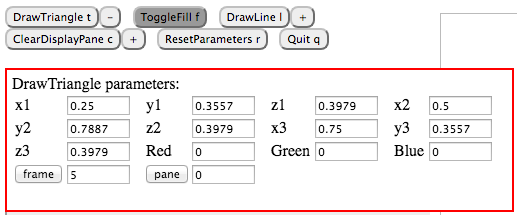
\includegraphics[width=0.75\textwidth]{pix/driver2.png}
\caption{example.c allows a user to draw lines and triangles. This figure shows the DrawTriangle drop down menu open.}
\label{fig:6-1}
\end{figure} 

If the ToggleFill button is highlighted then the triangle will be drawn unfilled. And if the ToggleFill button is not 
highlighted, the triangle will be filled. Press the ToggleFill button to toggle it.
The rest of the buttons are self explanatory. Figure \ref{fig:6-2} shows the result of drawing
4 unfilled triangles in 3D to create a tetrahedron. The image shows the tetrahedron after it has been rotated by
the user. The 4 vertices are drawn in $frame=5$ and positioned at $(0.25,0.3557,0.3979)$, $(0.5,0.7887,0.3979)$, 
$(0.75,0.3557,0.3979)$, $(0.5,0.5,0.8061)$. Note that $(0.5,0.5,0.5)$ is the center of rotation in $frame=5$.
In this example, the tetrahedron has edge length 0.5 and is centered at $(0.5,0.5,0.5)$.

\begin{figure}[H]
\centering
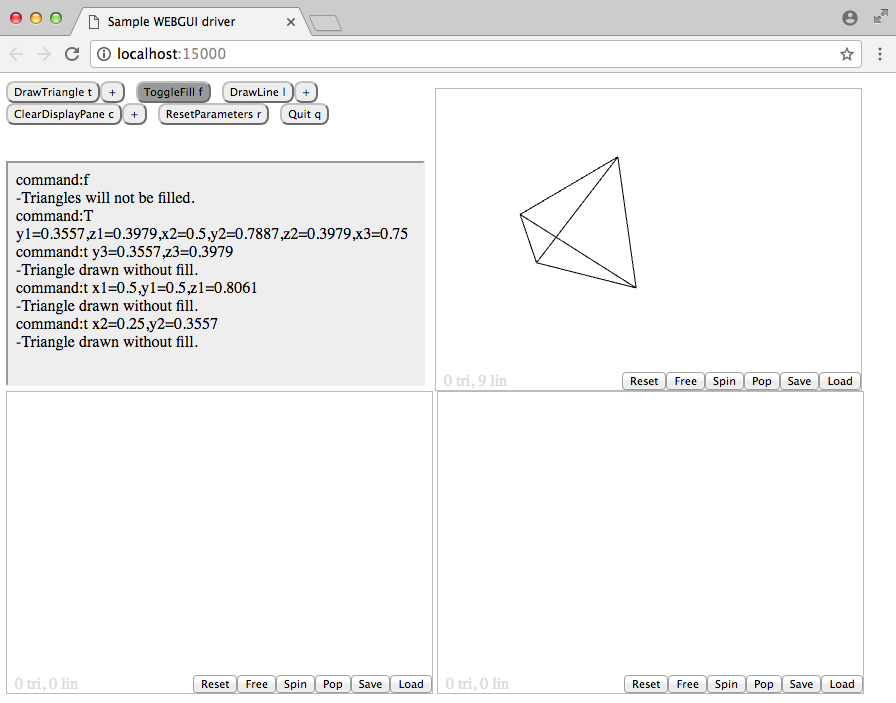
\includegraphics[width=0.75\textwidth]{pix/driver3.png}
\caption{example.c compiled with webgui.c. Then user draws a skeleton tetrahedron.}
\label{fig:6-2}
\end{figure} 

\section{Example driver source in C}
\begin{verbatim}
#include<stdio.h>
#include<stdlib.h>
#include<string.h>
#include<webgui.h>

/* general routines for any program using webgui.c */
void initParameterMap(char* str, int n);
char* extractVal(char* str, char key);
char processCommand(char* str);
void updateParameter(char* str, int index1, int index2);
char arrayGet(char* key);
int ipGet(char* key);
void ipSet(char* key, int value);
double rpGet(char* key);
void rpSet(char* key, double value);
char* spGet(char* key);
void spSet(char* key, char* value);
/* general variables */
int ct=0;
char** map_keys;
int* map_indices;
char* map_array;
double *rp_default, *rp;
int *ip_default, *ip;
char *sp_default, *sp;
char buffer[80];

/* program specific routines */
void drawTriangle();
void drawTriangleOutline();
void drawLine(int display);
void drawAllObjects(int pane);
void clearDisplay();
/* program specific variables */
char init[60][80]={
    "c c=DrawTriangle,k=t",
    "c c=ToggleFill, k=f",
    "c c=DrawLine,k=l",
    "c c=ClearDisplayPane, k=c",
    "c c=ResetParameters, k=r",
    "c c=Quit, k=q",
    "n n=x1, t=r, i=1, d=0.25",
    "n n=y1, t=r, i=2, d=0.25",
    "n n=z1, t=r, i=3, d=0.5",
    "n n=x2, t=r, i=4, d=0.75",
    "n n=y2, t=r, i=5, d=0.25",
    "n n=z2, t=r, i=6, d=0.5",
    "n n=x3, t=r, i=7, d=0.5",
    "n n=y3, t=r, i=8, d=0.75",
    "n n=z3, t=r, i=9, d=0.5",
    "n n=x4, t=r, i=10, d=0.25",
    "n n=y4, t=r, i=11, d=0.5",
    "n n=z4, t=r, i=12, d=0.5",
    "n n=x5, t=r, i=13, d=0.75",
    "n n=y5, t=r, i=14, d=0.5",
    "n n=z5, t=r, i=15, d=0.5",
    "n n=Red, t=i, i=1, d=0",
    "n n=Green, t=i, i=2, d=0",
    "n n=Blue, t=i, i=3, d=0",
    "n n=frame, t=i, i=4, d=5",
    "n n=pane, t=i, i=5, d=0",
    "r c=DrawTriangle, n=x1",
    "r c=DrawTriangle, n=y1",
    "r c=DrawTriangle, n=z1",
    "r c=DrawTriangle, n=x2",
    "r c=DrawTriangle, n=y2",
    "r c=DrawTriangle, n=z2",
    "r c=DrawTriangle, n=x3",
    "r c=DrawTriangle, n=y3",
    "r c=DrawTriangle, n=z3",
    "r c=DrawTriangle, n=Red",
    "r c=DrawTriangle, n=Green",
    "r c=DrawTriangle, n=Blue",
    "r c=DrawTriangle, n=frame",
    "r c=DrawTriangle, n=pane",
    "r c=DrawLine, n=x4",
    "r c=DrawLine, n=y4",
    "r c=DrawLine, n=z4",
    "r c=DrawLine, n=x5",
    "r c=DrawLine, n=y5",
    "r c=DrawLine, n=z5",
    "r c=DrawLine, n=Red",
    "r c=DrawLine, n=Green",
    "r c=DrawLine, n=Blue",
    "r c=DrawLine, n=frame",
    "r c=DrawLine, n=pane",
    "r c=ClearDisplayPane, n=pane",
    "s n=pane, v=0, l=\"0 top right\"",
    "s n=pane, v=1, l=\"1 bottom left\"",
    "s n=pane, v=2, l=\"2 bottom right\"",
    "s n=frame, v=1, l=\"1 all\"",
    "s n=frame, v=2, l=\"2 top right\"",
    "s n=frame, v=3, l=\"3 bottom right\"",
    "s n=frame, v=4, l=\"4 left\"",
    "s n=frame, v=5, l=\"5 rotate\""
};
float triangles[3][1000], lines[3][700];
int indexT[3]={0,0,0}, indexL[3]={0,0,0};
double red[3][200], green[3][200], blue[3][200];
int fill=1;

int main(int argc, char *argv[]){
    int i, offset=0; 
    char cmd, str[80];
    initParameterMap((char*)init,60);
    webinit((char*)init,60);
    websettitle("Sample WEBGUI driver");
    while (webstart(15000+offset)<0) offset++;
    while (1){
        webreadline(str);
        cmd = processCommand(str);
        if (cmd=='t'){
            if (fill==1){
                drawTriangle();
                webwriteline("-Triangle drawn with fill.");
            }
            else{
                drawTriangleOutline();
                webwriteline("-Triangle drawn without fill.");
            }
        }
        else if (cmd=='f'){
            fill *= -1;
            if (fill==1){
                webwriteline("-Triangles will be filled.");
                webbutton(0,"ToggleFill");
            }
            else {
                webwriteline("-Triangles will not be filled.");
                webbutton(1,"ToggleFill");
            }
        }
        else if (cmd=='l'){
            drawLine(1);
            webwriteline("-Line drawn.");
        }
        else if (cmd=='c'){
            clearDisplay();
            webwriteline("-Display pane cleared.");
        }
        else if (cmd=='r'){
            webupdate(ip_default,rp_default,sp_default);
            for (i=0;i<ct;i++){
                ip[i] = ip_default[i];
                rp[i] = rp_default[i];
                strcpy(sp+80*i, sp_default+80*i);
            }
            webwriteline("-Parameters reset.");
        }
        else if (cmd=='q'){
            webwriteline("-Quitting.");
            webstop();
            return 0;
        }
    }
    return 0;
}
void initParameterMap(char* str, int n){
    /* reads array of strings and initializes ip, rp, sp */
    /* and creates a map for accessing ip, rp, and sp */
    int i, index=0;
    for (i=0; i<n; i++) if (str[80*i]=='n') ct++;
    map_keys = (char**)malloc(ct * sizeof(char*));
    map_indices = (int*)malloc(ct * sizeof(int));
    map_array = (char*)malloc(ct * sizeof(char));
    rp_default = (double*)malloc(ct * sizeof(double));
    ip_default = (int*)malloc(ct * sizeof(int));
    sp_default = (char*)malloc(ct * sizeof(char*) * 80);
    rp = (double*)malloc(ct * sizeof(double));
    ip = (int*)malloc(ct * sizeof(int));
    sp = (char*)malloc(ct * sizeof(char*) * 80);
    for (i=0; i<ct; i++) map_keys[i] = (char*)malloc(20 * sizeof(char));
    for (i=0; i<n; i++)
    if (str[80*i]=='n'){
        strcpy(map_keys[index],extractVal(str+80*i,'n'));
        map_indices[index] = atoi(extractVal(str+80*i,'i'))-1;
        map_array[index] = *extractVal(str+80*i,'t');
        if (map_array[index]=='r'){
            rp_default[map_indices[index]] = atof(extractVal(str+80*i,'d'));
            rp[map_indices[index]] = rp_default[map_indices[index]];
        }
        else if (map_array[index]=='i'){
            ip_default[map_indices[index]] = atoi(extractVal(str+80*i,'d'));
            ip[map_indices[index]] = ip_default[map_indices[index]];
        }
        else if (map_array[index]=='s'){
            strcpy(sp_default+80*map_indices[index],extractVal(str+80*i,'d'));
            strcpy(sp+80*map_indices[index],sp_default+80*map_indices[index]);
        }
        index++;
    }
}
char* extractVal(char* str, char key){
    /* returns the value associated with key in str */
    buffer[0]=0;
    int index1 = 0, index2;
    while (index1<strlen(str)){
        if (str[index1]=='='){
            if (str[index1-1]==key){
                index2 = index1;
                while (index2<strlen(str) && str[index2]!=',') index2++;
                strncpy(buffer,str+index1+1,index2-index1-1);
                buffer[index2-index1-1]=0;
                break;
            }
        }
        index1++;
    }
    return buffer;
}
char processCommand(char* str){
    /* returns command char and updates parameters */
    int index1 = 1, index2 = 2;
    while (str[index2]!=' '){
        if (str[index2]==','){
            updateParameter(str,index1,index2);
            index1 = index2;
        }
        index2++;
    }
    if (index2>2) updateParameter(str,index1,index2);
    return str[0];
}
void updateParameter(char* str, int index1, int index2){
    /* parses str between index1 and index2 and updates parameter */
    int index3 = index1+1;
    while (str[index3]!='=') index3++;
    str[index2]=0; str[index3]=0;
    char ch = arrayGet(str+index1+1);
    if (ch=='r') rpSet(str+index1+1,atof(str+index3+1));
    else if (ch=='i') ipSet(str+index1+1,atoi(str+index3+1));
    else if (ch=='s') spSet(str+index1+1,str+index3+1);
    str[index2]=','; str[index3]='=';
}
char arrayGet(char* key){
    /* returns which array (ip, rp, sp) key belongs to */
    int i;
    char value = ' ';
    for (i=0; i<ct; i++) if (strcmp(map_keys[i],key)==0)
        value = map_array[i];
    return value;
}
int ipGet(char* key){
    int i, value = 0;
    for (i=0; i<ct; i++) if (strcmp(map_keys[i],key)==0)
        value = ip[map_indices[i]];
    return value;
}
void ipSet(char* key, int value){
    int i;
    for (i=0; i<ct; i++) if (strcmp(map_keys[i],key)==0)
        ip[map_indices[i]] = value;
    return;
}
double rpGet(char* key){
    int i;
    double value = 0;
    for (i=0; i<ct; i++) if (strcmp(map_keys[i],key)==0)
        value = rp[map_indices[i]];
    return value;
}
void rpSet(char* key, double value){
    int i;
    for (i=0; i<ct; i++) if (strcmp(map_keys[i],key)==0)
        rp[map_indices[i]] = value;
    return;
}
char* spGet(char* key){
    int i;
    buffer[0] = 0;
    for (i=0; i<ct; i++) if (strcmp(map_keys[i],key)==0)
        strcpy(buffer,sp + 80 * map_indices[i]);
    return buffer;
}
void spSet(char* key, char* value){
    int i;
    for (i=0; i<ct; i++) if (strcmp(map_keys[i],key)==0)
        strcpy(sp + 80 * map_indices[i],value);
    return;
}
void drawTriangle(){
    int i, j;
    char str[3], var[3]={'x','y','z'};
    int pane = ipGet("pane");
    /* save triangle data locally */
    triangles[pane][indexT[pane]*10 + 9] = ipGet("frame");
    for (int i=1;i<4;i++)
    for (int j=0;j<3;j++){
        sprintf(str,"%c%d",var[j],i);
        triangles[pane][indexT[pane]*10+3*(i-1)+j] = (float)rpGet(str);
    }
    red[pane][indexT[pane]] = ipGet("Red")/255.0;
    green[pane][indexT[pane]] = ipGet("Green")/255.0;
    blue[pane][indexT[pane]] = ipGet("Blue")/255.0;
    indexT[pane]++;
    /* draw all triangles and lines to pane */
    drawAllObjects(pane);
}
void drawTriangleOutline(){
    int i, j;
    double x4=rpGet("x4"), y4=rpGet("y4"), z4=rpGet("z4");
    double x5=rpGet("x5"), y5=rpGet("y5"), z5=rpGet("z5");
    char str[3], str2[3], var[3]={'x','y','z'};
    for (i=4;i<6;i++)
    for (j=0;j<3;j++){
        sprintf(str,"%c%d",var[j],i);
        sprintf(str2,"%c%d",var[j],i-3);
        rpSet(str, rpGet(str2));
    }
    drawLine(0);
    for (i=4;i<6;i++)
    for (j=0;j<3;j++){
        sprintf(str,"%c%d",var[j],i);
        sprintf(str2,"%c%d",var[j],i-2);
        rpSet(str, rpGet(str2));
    }
    drawLine(0);
    for (j=0;j<3;j++){
        sprintf(str,"%c4",var[j]);
        sprintf(str2,"%c1",var[j]);
        rpSet(str, rpGet(str2));
    }
    for (j=0;j<3;j++){
        sprintf(str,"%c5",var[j]);
        sprintf(str2,"%c3",var[j]);
        rpSet(str, rpGet(str2));
    }
    drawLine(1);
    rpSet("x4",x4); rpSet("y4",y4); rpSet("z4",z4);
    rpSet("x5",x5); rpSet("y5",y5); rpSet("z5",z5);
}
void drawLine(int display){
    int i, j;
    char str[3], var[3]={'x','y','z'};
    int pane = ipGet("pane");
    /* save line data locally */
    lines[pane][indexL[pane]*7 + 6] = ipGet("frame");
    for (int i=4;i<6;i++)
    for (int j=0;j<3;j++) {
        sprintf(str,"%c%d",var[j],i);
        lines[pane][indexL[pane]*7+3*(i-4)+j] = (float)rpGet(str);
    }
    red[pane][100+indexL[pane]] = ipGet("Red")/255.0;
    green[pane][100+indexL[pane]] = ipGet("Green")/255.0;
    blue[pane][100+indexL[pane]] = ipGet("Blue")/255.0;
    indexL[pane]++;
    /* draw all triangles and lines to pane */
    if (display==1) drawAllObjects(pane);
}
void drawAllObjects(int pane){
    int i, j;
    float x[3], y[3], z[3];
    websetcolors(200,red[pane],green[pane],blue[pane],pane);
    for (i=0;i<indexT[pane];i++){
        webframe((int)triangles[pane][i*10+9]);
        for (j=0;j<3;j++){
            x[j] = triangles[pane][10*i+3*j];
            y[j] = triangles[pane][10*i+3*j+1];
            z[j] = triangles[pane][10*i+3*j+2];
        }
        webfillflt(x,y,z,3,i+1);
    }
    for (i=0;i<indexL[pane];i++){
        webframe((int)lines[pane][i*7+6]);
        for (j=0;j<2;j++){
            x[j] = lines[pane][7*i+3*j];
            y[j] = lines[pane][7*i+3*j+1];
            z[j] = lines[pane][7*i+3*j+2];
        }
        weblineflt(x,y,z,2,i+101);
    }
    webgldisplay(pane);
}
void clearDisplay(){
    int pane = ipGet("pane");
    indexL[pane]=0;
    indexT[pane]=0;
    websetcolors(200,red[pane],green[pane],blue[pane],pane);
    webgldisplay(pane);
}
\end{verbatim}

\section{Example driver source in Fortran}



